\subsection{Presurgical evaluation}

\Ac{ASM} is normally used to treat epilepsy by decreasing the seizure frequency, but does not cure the underlying cause.
In roughly one third of the patients, \ac{ASM} does not adequately control seizures.
These patients are described as being medically refractory.
Half of the medically refractory epileptic patients have focal epilepsy, which may be treated by curative resective surgery.

The objective of resective epilepsy surgery is the complete resection or complete disconnection of the \ac{EZ}, which is defined as ``the area of cortex indispensable for the generation of clinical seizures'' \cite{rosenow_presurgical_2001}.
The surgery is performed if the \ac{EZ} can be definitely identified and is located in a part of the brain that may be removed without causing neurological, cognitive or neuropsychiatric deficit \cite{jobst_resective_2015}.

To locate the \ac{EZ}, \ac{EEG} and video-telemetry are acquired.
Analysis of these data may help lateralize or coarsely localize the \ac{EZ}.
Then, several preoperative imaging scans such as \ac{T1w} \ac{MRI} or \ac{T2w} \ac{FLAIR} \ac{MRI} are acquired to identify structural cerebral abnormalities, such as focal cortical dysplasia \cite{kabat_focal_2012}, hippocampal sclerosis \cite{thom_review_2014} or brain tumors.
If a structural lesion is found that is concordant with the results of \ac{EEG} and video-telemetry, the patient can be recommended for surgery \cite{duncan_brain_2016}.
However, 15 to 30\,\% of patients with focal epilepsy are \ac{MRI}-negative, meaning they have no distinct abnormalities visible from imaging or the abnormalities are discordant from video \ac{EEG} telemetry \cite{bien_characteristics_2009} (results are discordant when they suggest different \ac{EZ} localizations).
For example, an \ac{MRI} can show a lesion near the motor cortex, but \ac{EEG} shows abnormal activity in the occipital lobe.
In such cases, intracranial electrodes may be implanted to acquire \ac{iEEG} signals for precise localization of the \ac{EZ} (\cref{fig:electrodes}).

\begin{figure}[hbt!]
  \centering
  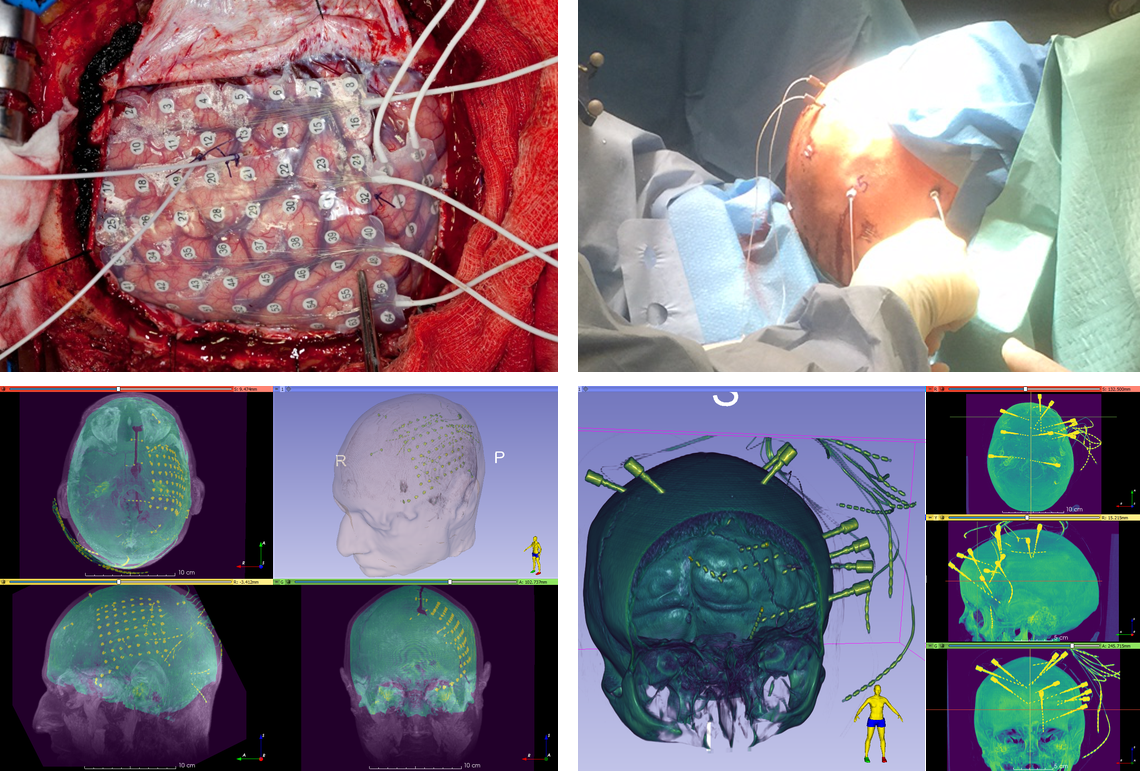
\includegraphics[width=\linewidth]{electrodes}
  \caption[Electrodes used for intracranial EEG]{
    Electrodes used for \acf{iEEG}.
    Left: subdural grid electrode;
    right: \acf{SEEG} depth electrodes.
    Top: intraoperative photos after electrode placement for each implantation procedure;
    bottom: volume renderings and \acfp{MIP} of post-implantation images.
    The skull is shown in green.
    The electrodes and cables are shown in yellow.
  }\label{fig:electrodes}
\end{figure}

The brain structures in which the electrodes are implanted are chosen by clinicians after interpretation of the aforementioned non-invasive data acquisition modalities, particularly seizure semiology, video-\ac{EEG} and \ac{MRI}.
However, there are significant variations in implantation strategies between centers, based on views regarding the relationship between semiological features and brain regions involved \cite{tufenkjian_seizure_2012}.
Therefore, tools to summarize findings across studies and highlight overall potential regions associated with a specific semiology may help standardize implantation approaches.

To determine an objective implantation plan for the \ac{iEEG} electrodes, we developed a data-driven tool that maps seizure semiologies to brain structures, using retrospective information from the literature (\cref{chap:svt}).
